\section{Поведение модели Изинга на блужданиях без самопересечений вблизи крит. температуры}

Критическая область - одна из сложнейших областей для изучения поведения любой термодинамической модели, как для теоретическим, так и экспериментальным способом. В частности, есть предположение, что модель Изинга на блужданиях без самопересечений вблизи крит. температуры (далее Изинг-блуждание) вблизи крит. температуры показывает схожесть в поведении с фазовым переходом жидкой/парообразной системы в области тройной точки, что даёт интересный повод для изучения данной области и расчётов критических экспонент с помощью симуляций Монте-Карло.

Определим приведённую температуру t как "расстояние" от критической температуры:

\begin{equation} \label{eq:redTemp}
    t = \frac{T - T_{C}}{T_{C}}
\end{equation}

T - текущая температура модели, $T_{C}$ - критическая температура. Тогда корреляционная длина при термодинамическом пределе (системе бесконечной длины) в критической области будет:

\begin{equation}\label{eq:CorLen}
    \xi \sim \mid t \mid ^{-\upsilon} 
\end{equation}
где $\upsilon$ - критическая экспонента

Также мы можем определить другие экспоненты - к примеру, в нормальной модели Изинга определяются экспоненты $\gamma$, $\alpha$ и $\beta$ для магнитной восприимчивости, темпоёмкости и намагниченности соответственно:

\begin{equation}
    \chi \sim \mid t \mid ^{-\gamma}
\end{equation}

\begin{equation}
    c \sim \mid t \mid ^{-\alpha}
\end{equation}

\begin{equation}
    m \sim \mid t \mid ^{-\beta}
\end{equation}

Рассмотрим случай квадрата намагниченности:

\begin{equation}
    m^{2} \sim \mid t \mid ^{-2\beta}
\end{equation}

Воспользовавшись \eqref{eq:CorLen}, избавимся от t:

\begin{equation}
    m^{2} \sim \xi ^{2\beta/\upsilon}
\end{equation}

учитывая поведение корреляционной длины в конечноразмерных системах (книга "Monte Carlo Methods in Statistical Physics", график 4.1 и стр. 232-233)\cite{NewBar}, мы можем представить функцию квадрата намагниченности в виде:

\begin{equation}\label{eq:m2_1}
    m^{2} = \xi ^{-2\beta/\upsilon} m_{02}(L/\xi)
\end{equation}

Где L - размер системы (для квадратной решётки кол-во спинов = L * L)

$m_{02}$ обладает следующими свойствами:

\begin{align*}
    m_{02}(x) = C,\ \ x >> 1 \\
    m_{02}(x) \sim x^{-2\beta/\upsilon},\ \ x \rightarrow 0
\end{align*}

Так как \eqref{eq:m2_1} содержит неизвестную нам корреляционную длину, преобразуем её с новой безразмерной функцией:

\begin{equation}
    \Tilde{m}_{02}(x) = x^{-2\beta} m_{02}(x^{\upsilon})
\end{equation}

Тогда получим:

\begin{equation}\label{eq:m2_2}
    m^{2} = L^{-2\beta/\upsilon} \Tilde{m}_{02}(L^{1/\upsilon}|t|)
\end{equation}

\subsection{Расчёты крит. экспонент при наблюдении коллапса данных}
Для того, чтобы найти крит. экспоненты $\beta$ и $\upsilon$, а также крит. температуру модели Изинга-блуждания, достаточно определить, при каких их значениях графики шкалирующих функций $\Tilde{m}_{02}$ для разных размеров L системы сливаются к как можно более однородному графику. Для этого значение шкал. функции расчитывается из \eqref{eq:m2_2}:

\begin{equation}\label{eq:m02}
    \Tilde{m}_{02} = L^{2\beta/\upsilon} m_{L}^{2}(t)
\end{equation}

Перед этим, был произведен расчёт зависимости квадрата намагниченности для квадратных решёток с длиннами L=300-1000 от температуры (https://github.com/kamilla0503/saw/tree/master/Ising/BC\cite{saw}). Наилучший коллапс данных наблюдался при:

\begin{align*}
    T_{C} = 1.1976 \\
    \beta = 0.125 \\
    \upsilon = 1.01
\end{align*}

\begin{figure}[!h]
    \centering
    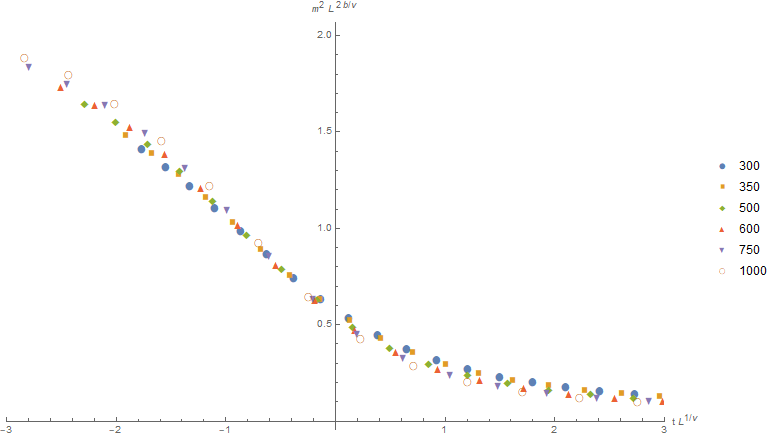
\includegraphics[width=100mm]{Sections/Images/DatColMagn2_3.png}
    \caption{График зависимости значений шкалирующей функции квадрата намагниченности от приведённой температуры при крит. экспонентах, обеспечивших наилучший коллапс данных}
    \label{fig:DatColM2_3}
\end{figure}

\subsection{Определение погрешностей измерений экспонент}

Разумеется, поскольку мы не можем численно определить качество коллапса данных, а лишь визуально определить при каких значениях он будет лучше, необходимо задать погрешность - область значений критических экспонент и температур, при которых качество коллапса данных наблюдаемой величины при измерении "на глаз" не меняется.

Таким образом, мы уточняем возможные критические значения для сравнения с расчётов в других источниках, для определения модели по её поведению.

\newpage

\begin{figure}[!h]
\begin{minipage}[h]{0.5\linewidth}
\center{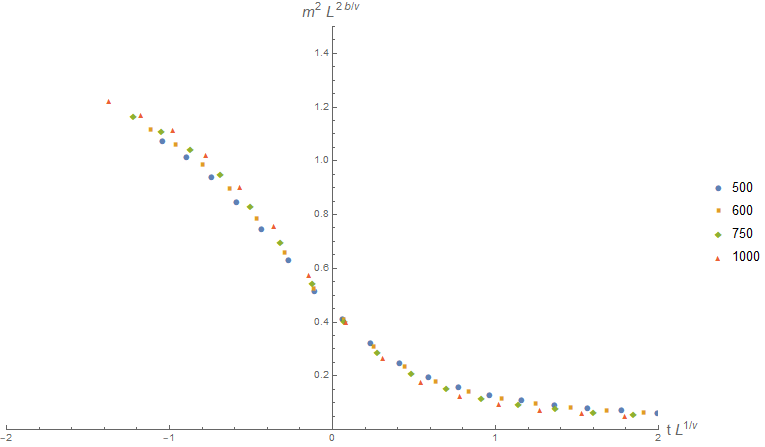
\includegraphics[width=0.9\linewidth]{Sections/Images/DataCollLowExp.png} \\ $\beta = 0.04,\ \nu = 0.8$}
\end{minipage}
\hfill
\begin{minipage}[h]{0.5\linewidth}
\center{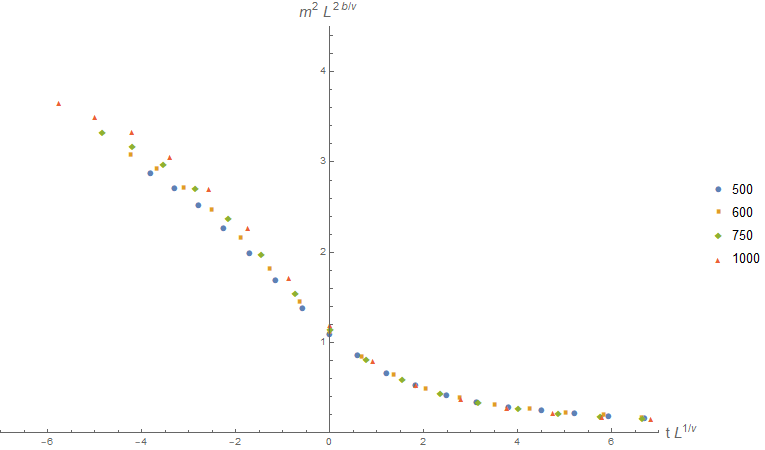
\includegraphics[width=0.9\linewidth]{Sections/Images/DataCollHighExp.png} \\ $\beta = 0.3,\ \nu = 1.2$}
\end{minipage}
\caption{Погрешность критических экспонент и их влияние на коллапс данных}
\label{ris:image1}
\end{figure}

Из графиков видно, что несмотря на колоссальное отличие от расчитанных из литературы\cite{NewBar} значений, качество коллапса данных для квадрата намагниченности едва отличается между графиками - отличие заключается лишь в их масштабе - что говорит о серьёзной погрешности данного метода для расчёта критических показателей модели.